% =====================================================================
%  Függelék: a módszer és a kiértékelés részletei (a 3. és 4. fejezetből)
% =====================================================================

\chapter{A módszer és a kiértékelés részletei}
\label{app-modszer}

Ez a függelék a 3. és a 4.~fejezet azon részleteit tartalmazza, amelyek a főszöveg megértéséhez nem
szükségesek, de a módszer és a mérés reprodukálásához igen. A paraméterek alapértékeit
\az{\ref{app-reprodukcio}}.~függelék foglalja össze.

% ---------------------------------------------------------------------
\section{Adatfajták életciklusa}
\label{app-eletciklus}
% ---------------------------------------------------------------------

\Az{\ref{tab:eletciklus}}.~táblázat a \Mimir{} által kezelt adatfajtákat, tárolási helyüket és
élettartamukat foglalja össze a szolgáltatások mai kódja szerint (vö.\ \ref{sec:zero}.~szakasz).

\begin{table}[htbp]
\centering
\caption[Adatfajták életciklusa a \Mimir{} rendszerben.]{Adatfajták életciklusa a \Mimir{} rendszerben,
a szolgáltatások mai kódja szerint. Az élettartamok környezeti változóval állíthatók; zárójelben az
alapérték.}
\label{tab:eletciklus}
\small
\begin{tabularx}{\textwidth}{@{}>{\raggedright\arraybackslash}p{3.4cm}>{\raggedright\arraybackslash}p{4.4cm}>{\raggedright\arraybackslash}X@{}}
\toprule
Adat & Tárolás & Élettartam \\
\midrule
Fájl, kinyert szöveg & a Wellspring és a RuneCarver memóriája & a kérés végéig; lemezre nem kerül \\
Darabok és beágyazásaik & Bifrost: memóriában futó Qdrant, egy közös gyűjtemény & a feladat végén (sikeres vagy hibás) törlődnek, és új dokumentum indexelésekor is \\
Prompt, nyers modellválasz & a Bifrost memóriája & a modellhívás végéig; kikapcsolt \code{LOCAL\_ONLY} mellett a szervermodellhez is eljut \\
Generált vizsga (vázlat) & a Bifrost memóriabeli feladattára; a szerkesztés a böngészőben & az indítástól 60 perc (\code{JOB\_TTL\_SECONDS}), utána a következő kérés törli \\
Jóváhagyott, mentett vizsga & Skald: PDF-fájl és SQLite-sor, csak kérésre & amíg az oktató nem törli, legfeljebb beállítható ideig (365 nap) \\
Audit napló & The Forge, PostgreSQL & csak metaadat és ujjlenyomat; óránkénti törlés (30 nap) \\
\bottomrule
\end{tabularx}
\end{table}

% ---------------------------------------------------------------------
\section{A GPU-memória becslése}
\label{app-vram}
% ---------------------------------------------------------------------

A szövegelőállítás közbeni memóriaigény három tag összege:
\begin{equation}
M \;=\; W \;+\; \mathrm{ctx}\cdot m_{kv} \;+\; M_0,
\label{eq:vram}
\end{equation}
ahol $W$ a kvantált súlyok mérete, $\mathrm{ctx}$ a kontextus hossza tokenben, $m_{kv}$ a
KV-gyorsítótár (a már feldolgozott tokenek kulcs- és értékvektorainak tára) tokenenkénti mérete, $M_0$
pedig a futtatókörnyezet többletigénye. Minden rétegben ($L$ réteg) minden kulcs--érték fejhez ($H_{kv}$
fej) egy kulcs- és egy értékvektort kell tárolni, egyenként $d_h$ elemmel és elemenként 2 bájttal. A
Qwen2.5-7B modellre~\cite{qwen25} ($L=28$, $H_{kv}=4$, $d_h=128$):
\begin{equation*}
m_{kv}=2\cdot 28\cdot 4\cdot 128\cdot 2\ \text{bájt}=57\,344\ \text{bájt}= 56\ \text{KiB},
\end{equation*}
így 8\,192 tokenes kontextusnál a gyorsítótár 448\,MiB, 16\,384 tokennél 896\,MiB, 32\,768 tokennél
1,75\,GiB. \Az{\ref{tab:budget}}.~táblázat több helyi generátorra mutatja a becslést. A Q4\_K\_M
kvantálás súlyonként átlagosan kb.\ 4,8 bitet használ, ezért a súlyok mérete a 16 bites változaténak
nagyjából harmada.

\begin{table}[htbp]
\centering
\caption[Becsült GPU-memóriaigény (8\,192 tokenes kontextus, Q4\_K\_M kvantálás).]{Becsült
GPU-memóriaigény 8\,192 tokenes kontextusnál, Q4\_K\_M kvantálással (kb.\ 4,8 bit/súly) és
$M_0\approx0{,}56$\,GiB többlettel. A súlyok a GGUF-fájlok GiB-ra átszámított mérete, $m_{kv}$ a
publikált architektúrákból számolt érték. A Gemma 3 12B sorában mért érték áll (lásd a szöveget).}
\label{tab:budget}
\small
\setlength{\tabcolsep}{4pt}
\begin{tabular}{@{}lccccc@{}}
\toprule
Modell & $L/H_{kv}$ & Súlyok & $m_{kv}$ & Összesen & Kártya \\
\midrule
Qwen2.5-3B  & 36/2 & 1,8\,GiB & 36\,KiB  & 2,6\,GiB  & 8\,GiB \\
Qwen2.5-7B  & 28/4 & 4,4\,GiB & 56\,KiB  & 5,4\,GiB  & 8\,GiB \\
Llama-3.1-8B~\cite{grattafiori2024llama3} (= PULI-LlumiX 8B) & 32/8 & 4,6\,GiB & 128\,KiB & 6,1\,GiB & 8\,GiB \\
Gemma 3 12B~\cite{gemma3} & 48/8 & 7,5\,GiB & ($\le$\,384\,KiB) & $\approx$\,7,8\,GiB (mért) & 12\,GiB \\
Qwen2.5-14B & 48/8 & 8,4\,GiB & 192\,KiB & 10,4\,GiB & 12\,GiB \\
\bottomrule
\end{tabular}
\end{table}

A PULI-LlumiX 8B~\cite{pulillumix} a Llama-3.1-8B architektúráját örökli, így memóriaigénye azonos vele.
A Gemma 3 12B-nél az egyszerű képlet túlbecsül: a modell rétegeinek többsége csak egy rövid, helyi
ablakra (\emph{sliding window}) figyel, és csak minden hatodik réteg lát a teljes kontextusra, ezért a
gyorsítótár jóval kisebb, mint $\mathrm{ctx}\cdot m_{kv}$. Ennél a modellnél ezért a mért értéket
használjuk: az Ollama 8\,192 tokenes kontextusnál kb.\ 7,8\,GiB-ot foglal.

% ---------------------------------------------------------------------
\section{A szemantikus darabolás vágási szabálya}
\label{app-darabolas}
% ---------------------------------------------------------------------

Két szomszédos mondat \emph{szemantikus távolsága}
\begin{equation}
\delta_i = 1-\cos\bigl(\mathbf{v}_i,\mathbf{v}_{i+1}\bigr),
\label{eq:delta}
\end{equation}
ahol $\mathbf{v}_i$ az $i$-edik mondat 768 dimenziós vektora (a mondat tokenjei vektorainak átlaga). A
darabolás ott vág, ahol $\delta_i$ meghaladja a $\tau$ vágási küszöböt; alapértelmezésben $\tau$ a
távolságok 85.~percentilise (az \arm{E5b}-ben az átlag $+\,1{,}5$ szórás). A célméret (1\,000 karakter)
túllépése után a hatásos küszöb $\tau/(\ell/1\,000)$, ahol $\ell$ az aktuális darab hossza karakterben;
egy kétszeres hosszúságú darab tehát már fele akkora távolságnál is lezárul.

% ---------------------------------------------------------------------
\section{A Bloom-szintek kiosztása}
\label{app-bloom}
% ---------------------------------------------------------------------

A kért nehézséghez egy Bloom-szint-eloszlás tartozik~\cite{anderson2001bloom}
(\ref{tab:bloom}.~táblázat), amelyet a \emph{legnagyobb maradék módszerével}
(Hamilton-módszer~\cite{balinski2001fair}) alakítunk egész darabszámokká: minden szint először a
kérdésszám és az arány szorzatának egészrészét kapja, a maradék helyeket pedig a legnagyobb törtrészű
szintek. Közepes nehézségnél $n=7$ kérdésre a szorzatok $(2{,}8;\,2{,}8;\,1{,}4)$, az egészrészek
$(2,2,1)$, a két maradék hely a két legnagyobb törtrészű szinthez kerül, így a kiosztás $(3,3,1)$. A
szinteket véletlenszerűen rendeljük a kérdéshelyekhez, a kész vizsgát pedig a könnyebbtől a nehezebb
felé rendezzük.

\begin{table}[htbp]
\centering
\caption{A nehézségi szintekhez rendelt Bloom-eloszlások és egy 10 kérdéses vizsga kiosztása.}
\label{tab:bloom}
\small
\begin{tabular}{@{}lccccc@{\qquad}c@{}}
\toprule
Nehézség & Emlékezés & Megértés & Alkalmazás & Elemzés & Értékelés & Kiosztás ($n=10$) \\
\midrule
Könnyű   & 0,5 & 0,5 & -- & -- & -- & (5, 5, 0, 0, 0) \\
Közepes  & -- & 0,4 & 0,4 & 0,2 & -- & (0, 4, 4, 2, 0) \\
Nehéz    & -- & -- & 0,3 & 0,4 & 0,3 & (0, 0, 3, 4, 3) \\
\bottomrule
\end{tabular}
\end{table}

% ---------------------------------------------------------------------
\section{A hibrid keresés}
\label{app-hibrid}
% ---------------------------------------------------------------------

Az \arm{E2h} a sűrű rangsort egy lexikális BM25-rangsorral~\cite{robertson2009bm25} egyesíti. A magyar
ragozás miatt a szavakat egyszerű \emph{előtagtövesítéssel} normalizáljuk: a hat karakternél hosszabb
szavakból az első hat karaktert tartjuk meg, így az „immunrendszer”, „immunrendszert”,
„immunrendszerben” alakok közös kulcsot kapnak. A két rangsort a reciprok rangfúzió~\cite{cormack2009rrf}
egyesíti; a $c$ darab pontszáma
\begin{equation}
\mathrm{RRF}(c)=\frac{1}{60+\mathrm{rang}_{\text{sűrű}}(c)}+\frac{1}{60+\mathrm{rang}_{\text{BM25}}(c)},
\label{eq:rrf}
\end{equation}
ahol a rang az 1-től számozott helyezés, a 60-as konstans pedig az irodalomban bevett érték, amely
csökkenti az első helyek túlzott súlyát.

% ---------------------------------------------------------------------
\section{Egy kérdéshely kitöltése}
\label{app-slot}
% ---------------------------------------------------------------------

\Az{\ref{alg:slot}}.~algoritmus az \arm{E2} egy kérdéshelyének kitöltését írja le
(vö.\ \ref{sec:verifier}.~szakasz). A hibák listája visszajelzésként („Az előző próbálkozás hibás volt,
javítsd: \dots”) a következő kísérlet promptjába kerül; ha a kulcs nem igazolt, a keresés két darabbal
bővül. Ha egy tartalékfogalommal sem sikerül, a \emph{legjobb} kísérlet (formailag helyes,
szivárgásmentes, legkevesebb hibájú) marad meg \emph{nem ellenőrzöttként} megjelölve; hibás formánál egy
\emph{javító} hívás pótolja a hiányzó disztraktorokat. \Az{\ref{fig:ellenorzo}}.~ábra ugyanezt
folyamatábraként mutatja.

\begin{figure}[htbp]
\centering
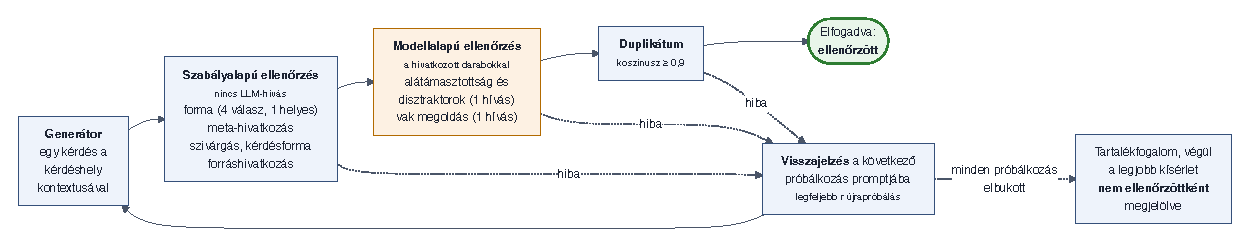
\includegraphics[width=\textwidth]{figures/d3_ellenorzo}
\caption[Az ellenőrző lánc visszacsatolással.]{Az ellenőrző lánc visszacsatolással. Az olcsó szabályalapú ellenőrzések előbb futnak; a hiba
szövege a következő generálási kísérlet promptjába kerül.}
\label{fig:ellenorzo}
\end{figure}

\begin{algorithm}[htbp]
\caption{Egy kérdéshely kitöltése visszacsatolással (\arm{E2}).}
\label{alg:slot}
\KwIn{kérdéshely $s$ (fogalom, típus, Bloom-szint); elfogadott kérdések $\mathcal{A}$; $k=3$; $r=1$}
\KwOut{kérdés $q$ és az \emph{ellenőrzött} jelző}
$q^{*}\gets\emptyset$\;
\ForEach{fogalom $c \in \bigl(s.\mathit{fogalom},\ \text{az első tartalékfogalom}\bigr)$}{
  $h\gets\emptyset$;\quad $k'\gets k$\;
  \For{$t=0,\dots,r$}{
    $K\gets$ \textsc{Kontextus}$(c,k')$ \tcp*{$\le$ 6\,000 karakter}
    $q\gets$ \textsc{Generál}$(s,c,K,\mathcal{A},h)$ \tcp*{$h$: az előző hibák}
    $h\gets$ \textsc{Ellenőriz}$(q,K)\ \cup$ \textsc{Duplikátum}$(q,\mathcal{A})$\;
    \lIf{$h=\emptyset$}{\KwRet $(q,\ \text{igaz})$}
    $q^{*}\gets$ a jobb $q^{*}$ és $q$ közül\;
    \lIf{a kulcs nem igazolt}{$k'\gets k'+2$}
  }
}
\lIf{$q^{*}$ formája hibás}{$q^{*}\gets$ \textsc{Javít}$(q^{*})$}
\KwRet $(q^{*},\ \text{hamis})$\;
\end{algorithm}

% ---------------------------------------------------------------------
\section{A fogalomgráf}
\label{app-graf}
% ---------------------------------------------------------------------

Az \arm{E3} a darabokat legfeljebb 3\,000 karakteres kötegekbe csoportosítja, és kötegenként egy
hívásban kinyeri a fogalmakat (definícióval, szülőfogalommal, darabazonosítókkal), a rövid tényeket és a
fogalmak közötti kapcsolatokat (\emph{fajtája}, \emph{része}, \emph{okozza}, \emph{ellentéte} stb.). A
nagyon hasonló nevű fogalmakat (névbeágyazásuk koszinusz-hasonlósága legalább 0,92) összevonja, ami a
ragozott alakokat is egyesíti. A fogalmakat a
$\mathrm{cent}(v)=\text{kapcsolatok száma}+\tfrac12\cdot\text{darabok száma}+\tfrac12\cdot\text{tények
száma}$ centralitás szerint rendezi, és ez a lista lép a tervező helyébe. A generátor
disztraktor-ötletként a fogalom \emph{testvérfogalmait} kapja (azonos szülőjű fogalmakat, például a
„T-sejt” mellett a „B-sejtet”), a kontextus pedig a szomszédos fogalmak darabjaival bővül.

% ---------------------------------------------------------------------
\section{Az adatkészlet}
\label{app-adatkeszlet}
% ---------------------------------------------------------------------

Az \code{eval-v1} adatkészlet 39 dokumentumból áll, három forrásból (\ref{tab:adatkeszlet}.~táblázat).
Minden referenciakérdéshez rendelkezésre áll a forrásszakasz \emph{és} a választ igazoló mondat, mert a
keresési mutatók ezt igénylik. A három saját szöveghez négy-négy kézzel írt referenciakérdés tartozik;
az importált forrásokból csak azokat a kérdéseket tartottuk meg, amelyek igazoló mondata szó szerint
szerepel a dokumentumban.

\begin{table}[htbp]
\centering
\caption[Az \code{eval-v1} adatkészlet és a fő vizsgálatban használt része.]{Az \code{eval-v1} adatkészlet és a fő vizsgálatban használt része. R/K/H: rövid
($\le$\,6\,000), közepes (6\,000--25\,000) és hosszú (25\,000--90\,000 karakteres) dokumentumok.}
\label{tab:adatkeszlet}
\small
\begin{tabular}{@{}llrcrccl@{}}
\toprule
 & & \multicolumn{3}{c}{\code{eval-v1}} & \multicolumn{2}{c}{Fő vizsgálat} & \\
\cmidrule(lr){3-5}\cmidrule(lr){6-7}
Forrás & Nyelv & Dok. & R/K/H & Ref.\ kérdés & Dok. & R/K/H & Licenc \\
\midrule
Saját oktatási szövegek & magyar & 3 & 3/0/0 & 12 & 3 & 3/0/0 & saját \\
OpenStax, EduQG & angol & 12 & 4/4/4 & 74 & 3 & 1/1/1 & CC BY 4.0 \\
Wikipédia, MILQA & magyar & 24 & 8/8/8 & 240 & 24 & 8/8/8 & CC BY-SA 4.0 \\
\midrule
Összesen & & 39 & 15/12/12 & 326 & 30 & 12/9/9 & \\
\bottomrule
\end{tabular}
\end{table}

% ---------------------------------------------------------------------
\section{A konfigurációk egytényezős fája}
\label{app-karok}
% ---------------------------------------------------------------------

\Az{\ref{fig:kiserleti-terv}}.~ábra \az{\ref{tab:karok}}.~táblázat konfigurációit mutatja: minden
konfiguráció pontosan egy tényezőben tér el a szülőjétől (vö.\ \ref{sec:karok}.~szakasz).

\begin{figure}[htbp]
\centering
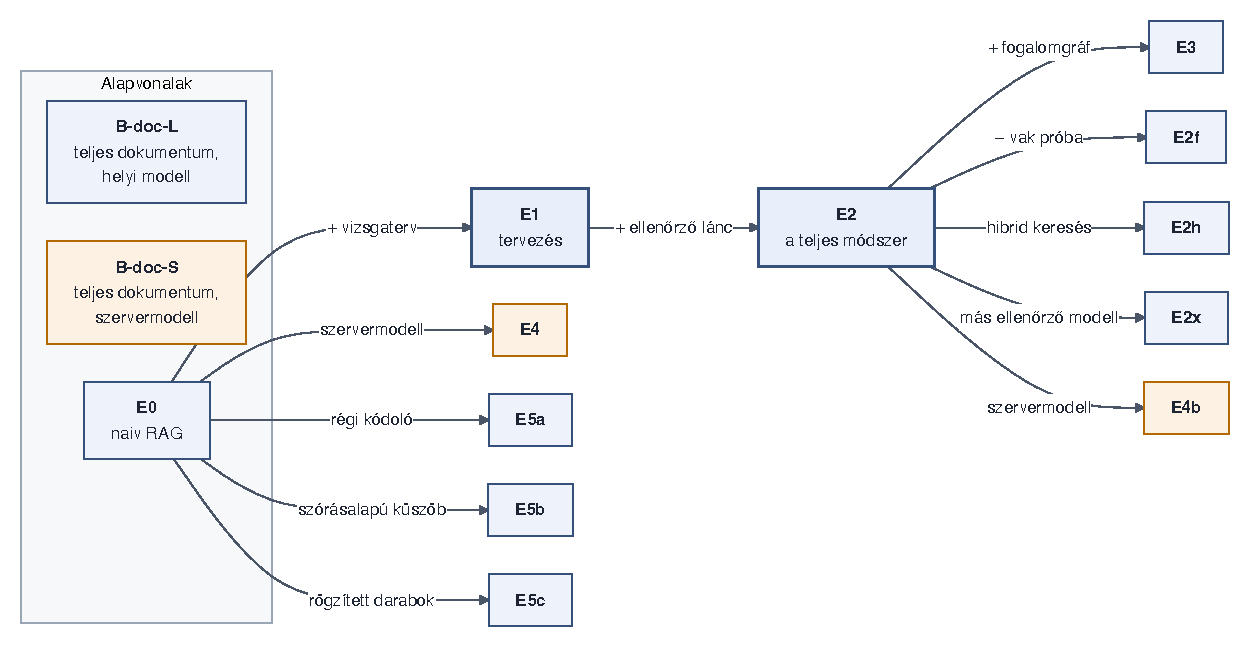
\includegraphics[width=0.9\textwidth]{figures/d5_kiserleti_terv}
\caption{A konfigurációk egytényezős fája: minden él egyetlen tényező megváltoztatása.}
\label{fig:kiserleti-terv}
\end{figure}

% ---------------------------------------------------------------------
\section{Az oktatói értékelés protokollja}
\label{app-oktatoi}
% ---------------------------------------------------------------------

Alapbeállításban a kiválasztott konfigurációkból konfigurációnként 30 kérdést mintavételezünk (előbb
minden dokumentumból egyet), 3 értékelővel és 10 közös kalibrációs kérdéssel. Az xlsx-lapok vakok (a
konfiguráció neve nem szerepel, a sorrend értékelőnként eltérő véletlen sorrend); minden kérdés mellett
egy, minden konfigurációnál azonos módon kiválasztott forrásrészlet áll, a rubrika a bíróéval azonos. Az
oktatók egymás közötti egyezését szempontonként Krippendorff-$\alpha$-val~\cite{krippendorff2004}, a bíró
és az oktatók egyezését Spearman-féle rangkorrelációval és Krippendorff-$\alpha$-val, a bináris
ítéletekre (a bíró „alátámasztott” ítélete vs.\ oktatói helyesség $\ge 4$) Cohen-$\kappa$-val mérjük.

% ---------------------------------------------------------------------
\section{A mutatók részletes definíciói}
\label{app-mutatok}
% ---------------------------------------------------------------------

\paragraph{Lefedettség.} Minden kérdéshez (törzs és kulcs együtt) megkeressük a beágyazás szerint
legközelebbi darabot:
\begin{equation}
\mathrm{Lef}=\frac{\text{a kérdésekhez legközelebbi különböző darabok száma}}{K},
\label{eq:cov}
\end{equation}
ahol $K$ a dokumentum darabjainak száma. Egy tízkérdéses vizsga lefedettsége legfeljebb $10/K$, így egy
százdarabos dokumentumon legfeljebb 10\,\%.

\paragraph{Szivárgás és nem kérdő törzs.} \emph{Szivárgás}, ha a legalább háromszavas kulcs szavainak
legalább 80\,\%-a a törzsben is szerepel (egy egyszavas tulajdonnév így nem ad téves jelzést); \emph{nem
kérdés} a törzs, ha sem kérdőjelre, sem kettőspontra nem végződik.

\paragraph{További mutatók.} A \emph{duplikátumráta} azon kérdéspárok aránya, amelyek
koszinusz-hasonlósága meghaladja a 0,9-et; a \emph{meta-hivatkozás} aránya azoké, amelyek „a szöveg
szerint” jellegű fordulatot tartalmaznak. A \emph{keresési találati arány} (recall@3) azt méri, hogy a
referenciakérdésekkel futtatott keresés első három találata között szerepel-e az igazoló mondatot
tartalmazó darab; a \emph{tematikus hasonlóság} azt, hogy a referenciakérdések mekkora részéhez van
beágyazás szerint közeli generált kérdés. \emph{Költségmutató} a futási idő (szakaszonként), a
modellhívások és tokenek száma, valamint a GPU-memória alapszintje és csúcsa.

% ---------------------------------------------------------------------
\section{A statisztikai eljárások részletei}
\label{app-statisztika}
% ---------------------------------------------------------------------

\paragraph{Hatásnagyság.} A páros Wilcoxon-próba~\cite{wilcoxon1945} mellett a hatás nagysága a
rangbiszeriális korreláció~\cite{kerby2014}:
\begin{equation}
r_{rb}=\frac{W^{+}-W^{-}}{W^{+}+W^{-}},
\label{eq:rrb}
\end{equation}
ahol $W^{+}$ és $W^{-}$ a pozitív, illetve a negatív különbségek rangösszege; $+1$, ha az új
konfiguráció minden dokumentumon jobb, $-1$, ha mindenütt rosszabb.

\paragraph{A minimális mintaméret.} $D$ dokumentum esetén a legkisebb elérhető kétoldali $p$-érték
$2\cdot 2^{-D}$, amelyet akkor kapunk, ha minden különbség azonos előjelű. Hat dokumentumnál ez $0{,}031$,
ötnél $0{,}0625$: hat dokumentum a legkisebb szám, amelyen egy összevetés egyáltalán szignifikáns
lehet. Holm-korrekció~\cite{holm1979} után a hat előre rögzített összehasonlítás közül a legkisebb
$p$-értéket 6-tal szorozzuk, így hat dokumentumnál a legkisebb elérhető korrigált érték $0{,}19$.

\paragraph{Egyezés és az ellenőrző mint osztályozó.} Két igen/nem ítéletsor (például az ellenőrzőé és a
bíróé) egyezését Cohen-$\kappa$-val~\cite{cohen1960kappa} mérjük:
\begin{equation}
\kappa=\frac{p_o-p_e}{1-p_e},
\label{eq:kappa}
\end{equation}
ahol $p_o$ a megfigyelt, $p_e$ a véletlenül várható egyezési arány; $\kappa=0$ a véletlen szintje,
$\kappa=1$ a teljes egyezés, az értelmezés Landis és Koch~\cite{landis1977} skáláját követi. Az ellenőrző
lánc minden kérdést \emph{átengedett} vagy \emph{megjelölt} kategóriába sorol; a bíró alátámasztottsági
ítéletét referenciának tekintve
\begin{equation}
\text{pontosság}=\frac{\text{átengedett és alátámasztott}}{\text{átengedett}},\qquad
\text{felidézés}=\frac{\text{átengedett és alátámasztott}}{\text{alátámasztott}}.
\label{eq:precrec}
\end{equation}
